\documentclass[a4paper, 12pt]{article}

\usepackage{hyperref}
\usepackage[warn]{mathtext}
\usepackage[utf8]{inputenc}
\usepackage[T2A]{fontenc}
\usepackage[english,russian]{babel}
\usepackage{multirow}
\usepackage{float}
\restylefloat{table}
\usepackage{amsmath,amsfonts,amssymb,amsthm,mathtools}
\usepackage{indentfirst}
\DeclareSymbolFont{T2Aletters}{T2A}{cmr}{m}{it}
\usepackage{ gensymb }
\mathtoolsset{showonlyrefs=true}
\usepackage{euscript}
\usepackage{mathrsfs}
\usepackage[left=2cm,right=2cm,top=2cm,bottom=2cm]{geometry}
\usepackage{graphicx}
\usepackage{wrapfig}
\usepackage[rgb]{xcolor}
\hypersetup{
colorlinks=true,
urlcolor=blue
}
\usepackage{tikz}

\title{Лабораторная работа}
\author{Гисич Арсений Б03-101}
\date{2023}

\begin{document}

	\begin{center}
		{\large МОСКОВСКИЙ ФИЗИКО-ТЕХНИЧЕСКИЙ ИНСТИТУТ (НАЦИОНАЛЬНЫЙ ИССЛЕДОВАТЕЛЬСКИЙ УНИВЕРСИТЕТ)}
	\end{center}
	\vspace{5 cm}
	{\Large
		\begin{center}
			{\bf Лабораторная работа 5.1.3}\\[0.2 cm]
			Эффект Рамзауэра
		\end{center}
	}
	\vspace{4 cm}
	\begin{flushright}
		{\Large Выполнили: \\
			\vspace{0.2 cm}
			Гисич Арсений \\
            Вазюля Василиса \\ 
			\vspace{0.2 cm}
			Б03-101 \\}
	\end{flushright}
	\vspace{8 cm}
	\begin{center}
		Долгопрудный\\[0.1 cm]
		2023
	\end{center}
\thispagestyle{empty}

\section{Аннотация}

В данной работе исследуется энергетическая зависимость вероятности рассеяния электронов атомами ксенона, определяются энергии электронов, при которых наблюдается <<просветление>> ксенона, и оценивается размер его внешней электронной оболочки.

\section{Теоретические сведения}

\begin{wrapfigure}{}{0.3\textwidth}
	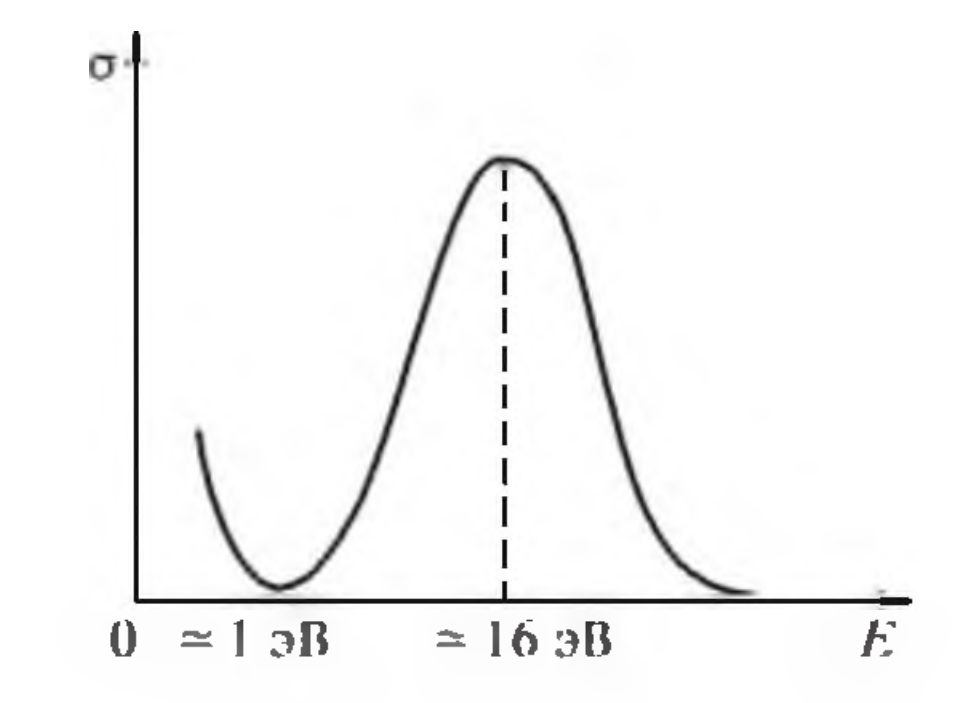
\includegraphics[width=1.0\linewidth]{Screenshot_1}
	\caption{Качественная картина результатов измерения упругого рассеяния электронов в аргоне}
	\label{fig:screenshot1}
\end{wrapfigure}

Эффективное сечение реакции -- это величина, характеризующая вероятность перехода системы двух сталкивающихся частиц в результате их рассеяния (упругого или неупругого) в определенное конечное состояние. Сечение $ \sigma $ равно отношению числа $ N $ таких переходов в единицу времени к плотности потока рассеиваемых частиц $ n v $, падающих на мишень, т. е. к числу частиц, проходящих в единицу времени через единичную площадку, перпендикулярную к их скорости $ v $ ($ n $ -- плотность числа падающих частиц).

\begin{equation}\label{eq:sigma}
	\sigma = \frac{N}{n v}.
\end{equation}
Таким образом, сечение имеет размерность площади.

Качественно результат экспериментов Рамзауэра при энергии электронов порядка десятков эВ показан на рис. \ref{fig:screenshot1}.
По мере уменьшения энергии электрона от нескольких десятков электрон-вольт поперечное сечение его упругого рассеяния растет. Однако при энергиях меньше 16 эВ в случае аргона сечение начинает уменьшаться, а при $ E \sim 1 $ эВ практически равно нулю, т. е. аргон становится прозрачным для электронов. При дальнейшем уменьшении энергии электронов сечение рассеяния опять начинает возрастать. Это поведение поперечного сечения свойственно не только атомам аргона, но и атомам всех инертных газов. Такое поведение электронов нельзя объяснить с позиций классической физики. Объяснение этого эффекта потребовало учета волновой природы электронов. Схема эксперимента Рамзауэра показана, на рис. \ref{fig:screenshot2}.

\begin{figure}[h!]
	\centering
	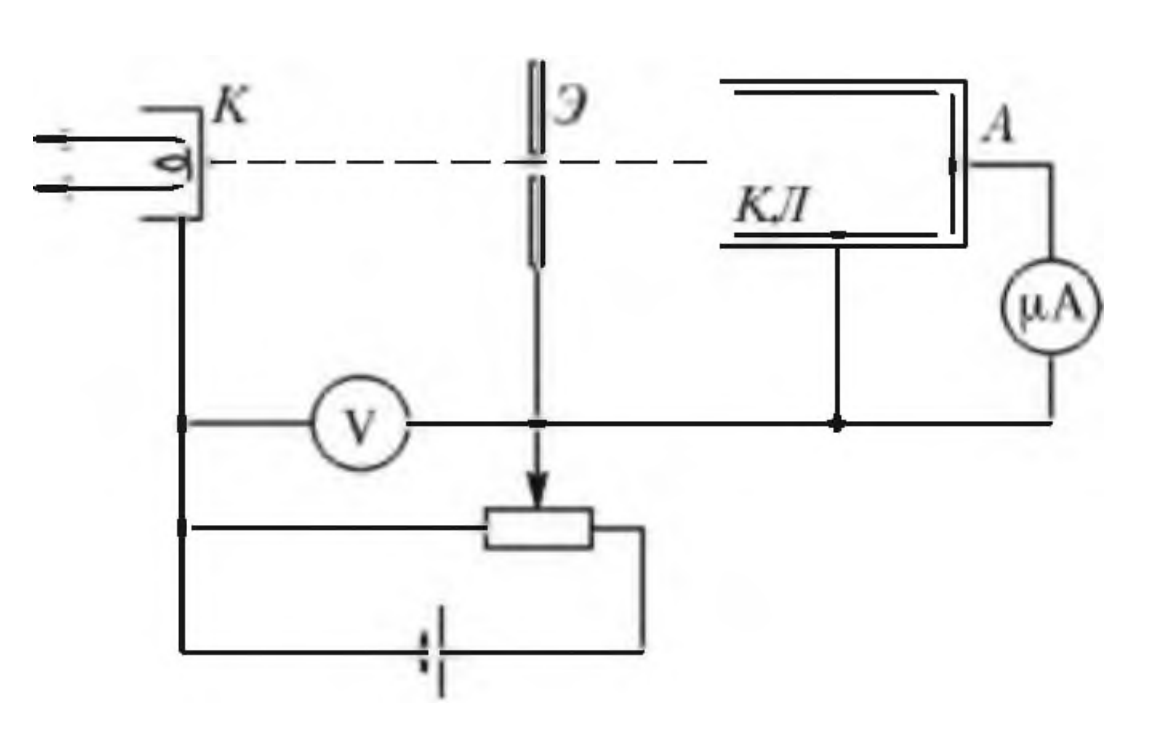
\includegraphics[width=0.5\linewidth]{Screenshot_2}
	\caption{Схема установки для измерения сечения рассеяния электронов в газах}
	\label{fig:screenshot2}
\end{figure}

С точки зрения квантовой теории, внутри атома потенциальная энергия налетающего электрона $ U $ отлична от нуля, скорость электрона изменяется, становясь равной $ v' $ в соответствии с законом сохранения энергии
\begin{equation*}
	E = \frac{m v^2}{2} = \frac{m v'^2}{2}+ U,
\end{equation*}
а значит, изменяется и длина его волны де Бройля. Таким образом, по отношению к электронной волне атом ведет себя как преломляющая среда с относительным показателем преломления
\begin{equation*}
	n = \frac{\lambda}{\lambda'} = \sqrt{1-\frac{U}{E}}.
\end{equation*}

Коэффициент прохождения электронов максимален при условии
\begin{equation}\label{eq:at}
	\sqrt{\frac{2 m (E+U_0)}{\hbar^2}}l = \pi n;\; n \in \mathbb{N}_1,
\end{equation}
где $ U_0 $ -- глубина потенциальной ямы.

Это условие легко получить, рассматривая интерференцию электронных волн де Бройля в атоме. Движущемуся электрону соответствует волна де Бройля, длина которой определяется соотношением $ \lambda = h/m v $. Если кинетическая энергия электрона невелика, то $ E = m v^2/2 $ и $ \lambda = h/\sqrt{2 m E} $. При движении электрона через атом длина волны де Бройля становится меньше и равна $ \lambda' = h/\sqrt{2 m (E+U_0)} $ где $ U_0 $ — глубина атомного потенциала. При этом, волна де Бройля отражается от границ атомного потенциала, т. е. от поверхности атома, и происходит интерференция прошедшей через атом волны 1 и волны 2, отраженной от передней и задней границы атома (эти волны когерентны). Прошедшая волна 1 усилится волной 2, если геометрическая разность хода между ними $ \Delta = 2 l = \lambda' $, что соответствует условию первого интерференционного максимума, т. е. при условии
\begin{equation}\label{eq:condition}
	2 l = \frac{h}{\sqrt{2 m (E_1 + U_0)}}
\end{equation}
Прошедшая волна ослабится при условии
\begin{equation}\label{eq:condition2}
	2 l = \frac{3}{2}\frac{h}{\sqrt{2 m (E_1 + U_0)}}
\end{equation}

Из \eqref{eq:condition} и \eqref{eq:condition2}, можно получить
\begin{equation}\label{eq:radius}
	l = \frac{h \sqrt{5}}{\sqrt{32 m (E_2-E_1)}}.
\end{equation}
Оттуда же можно найти эффективную глубину потенциальной ямы атома:
\begin{equation}\label{eq:atomPit}
	U_0 = \frac{4}{5}E_2-\frac{9}{5} E_1.
\end{equation}

Уравнение вольт-амперной характеристики тиратрона:
\begin{equation}\label{eq:VAH}
	I_а = I_0 \exp (-C \omega (V));\; C = L n_а \Delta_а,
\end{equation}
где $ I_0 = e N_0 $ -- ток катода, а $ I_а = e N_а $ -- ток анода.
Отсюда определяется вероятность рассеяния электрона в зависимости от его энергии:
\begin{equation}\label{eq:probable}
	\omega (V) = -\frac{1}{C} \ln \frac{I_а(V)}{I_0}.
\end{equation}

\section{Методика измерений}

Схема экспериментальной установки отображена на рис. \ref{fig:screenshot3}.
\begin{figure}[h!]
	\centering
	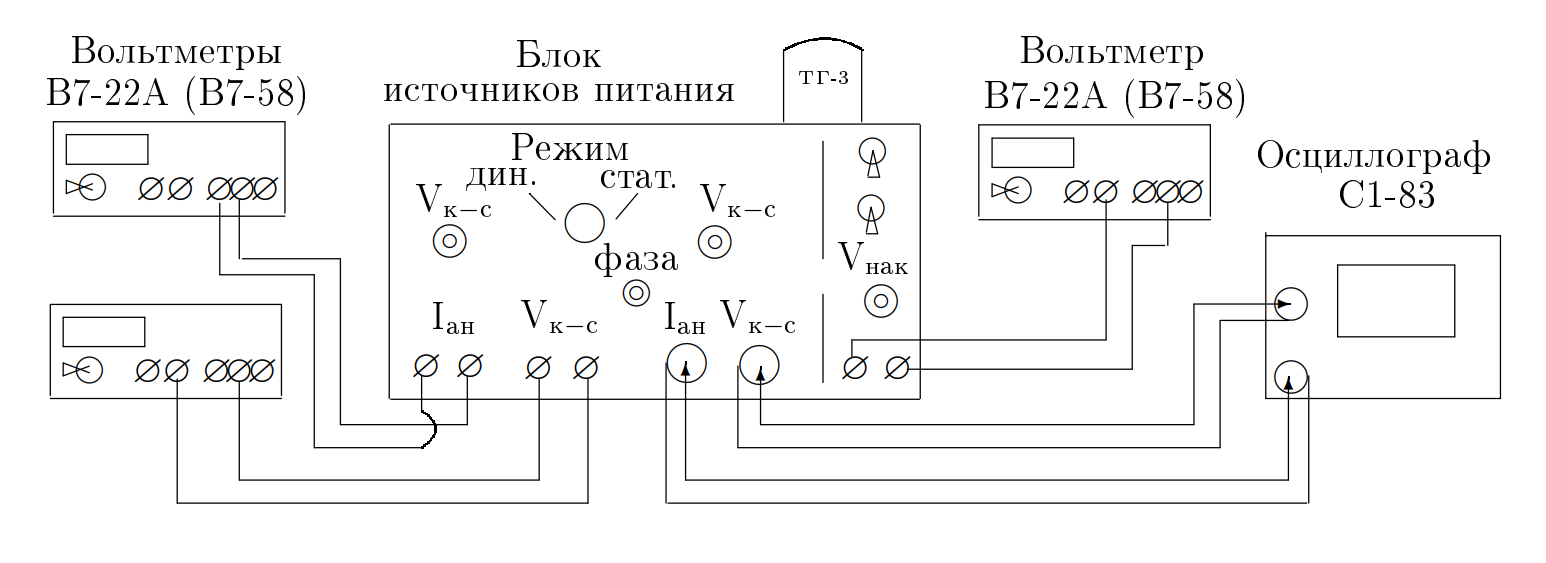
\includegraphics[width=1.0\linewidth]{Screenshot_3}
	\caption{Схема экспериментальной установки}
	\label{fig:screenshot3}
\end{figure}

В данной работе для изучения эффекта Рамзауэра используется
тиратрон ТГЗ-01/1.3Б, заполненный инертным газом. Электроны, эмитируемые катодом тиратрона, ускоряются напряжением $ V $, приложенным между катодом и ближайшей к нему сеткой. Затем электроны рассеиваются на атомах инертного газа (ксенона). Все сетки соединены между собой и имеют одинаковый потенциал, примерно равный потенциалу анода. Поэтому между первой сеткой и анодом практически нет поля. Рассеянные электроны отклоняются в сторону и уходят на сетку, а оставшаяся часть электронов достигает анода и создаёт анодный ток $ I_а $. Таким образом, поток электронов $ N(x) $ (т. е. число электронов, проходящих через поперечное сечение лампы в точке $ x $ в единицу времени) уменьшается с ростом $ x $ от начального значения $ X $ y катода (в точке $ x=0 $) до некоторого значения $ N_а $ у анода (в точке
$ x=L $).

\section{Используемое оборудование}

\begin{enumerate}
    \item вольтметры;
    \item блок питания;
    \item тиратрон ТГЗ;
    \item осциллограф;
\end{enumerate}

\section{Результаты измерений и обработка данных}

\subsection{Динамический режим}

По результатам измерений в динамическом режиме оценим размер электронной оболочки атома инертного газа по формулам \eqref{eq:condition} и \eqref{eq:condition2}.

Осциллограммы для двух значений $V_{накала}$ представлены на рис.~\ref{fig:osc}.
\begin{figure}[h]
		\begin{minipage}[h]{0.5\linewidth}
			\center{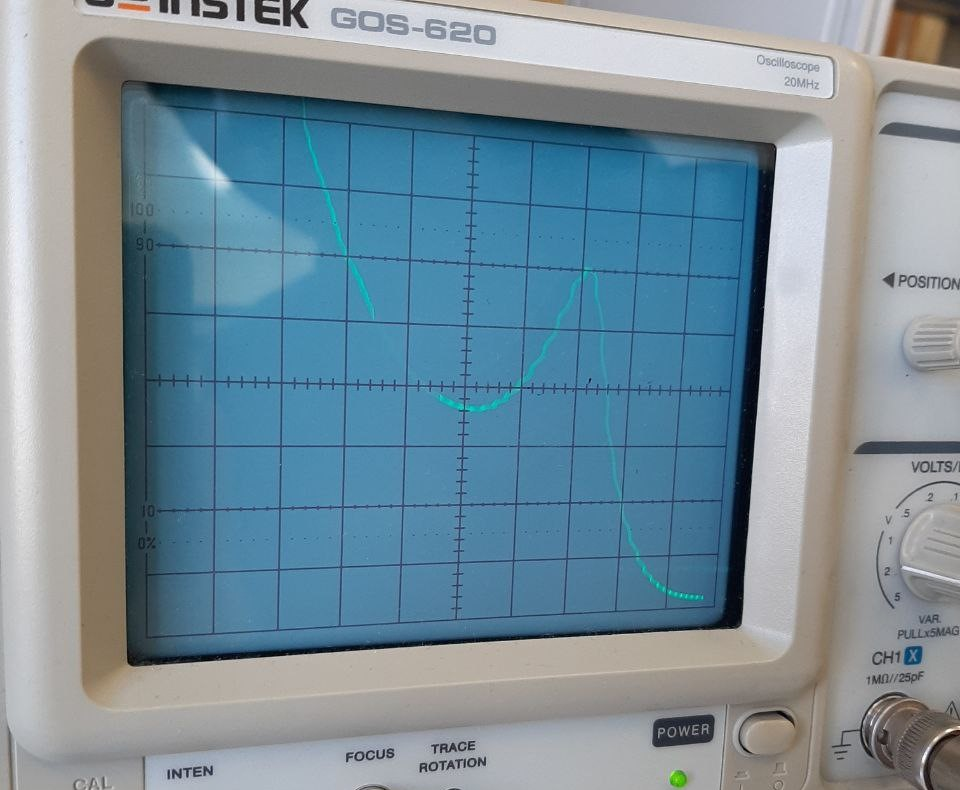
\includegraphics[width=0.9\linewidth]{osc1.jpg} \\ a)}
		\end{minipage}
		\hfill
		\begin{minipage}[h]{0.5\linewidth}
			\center{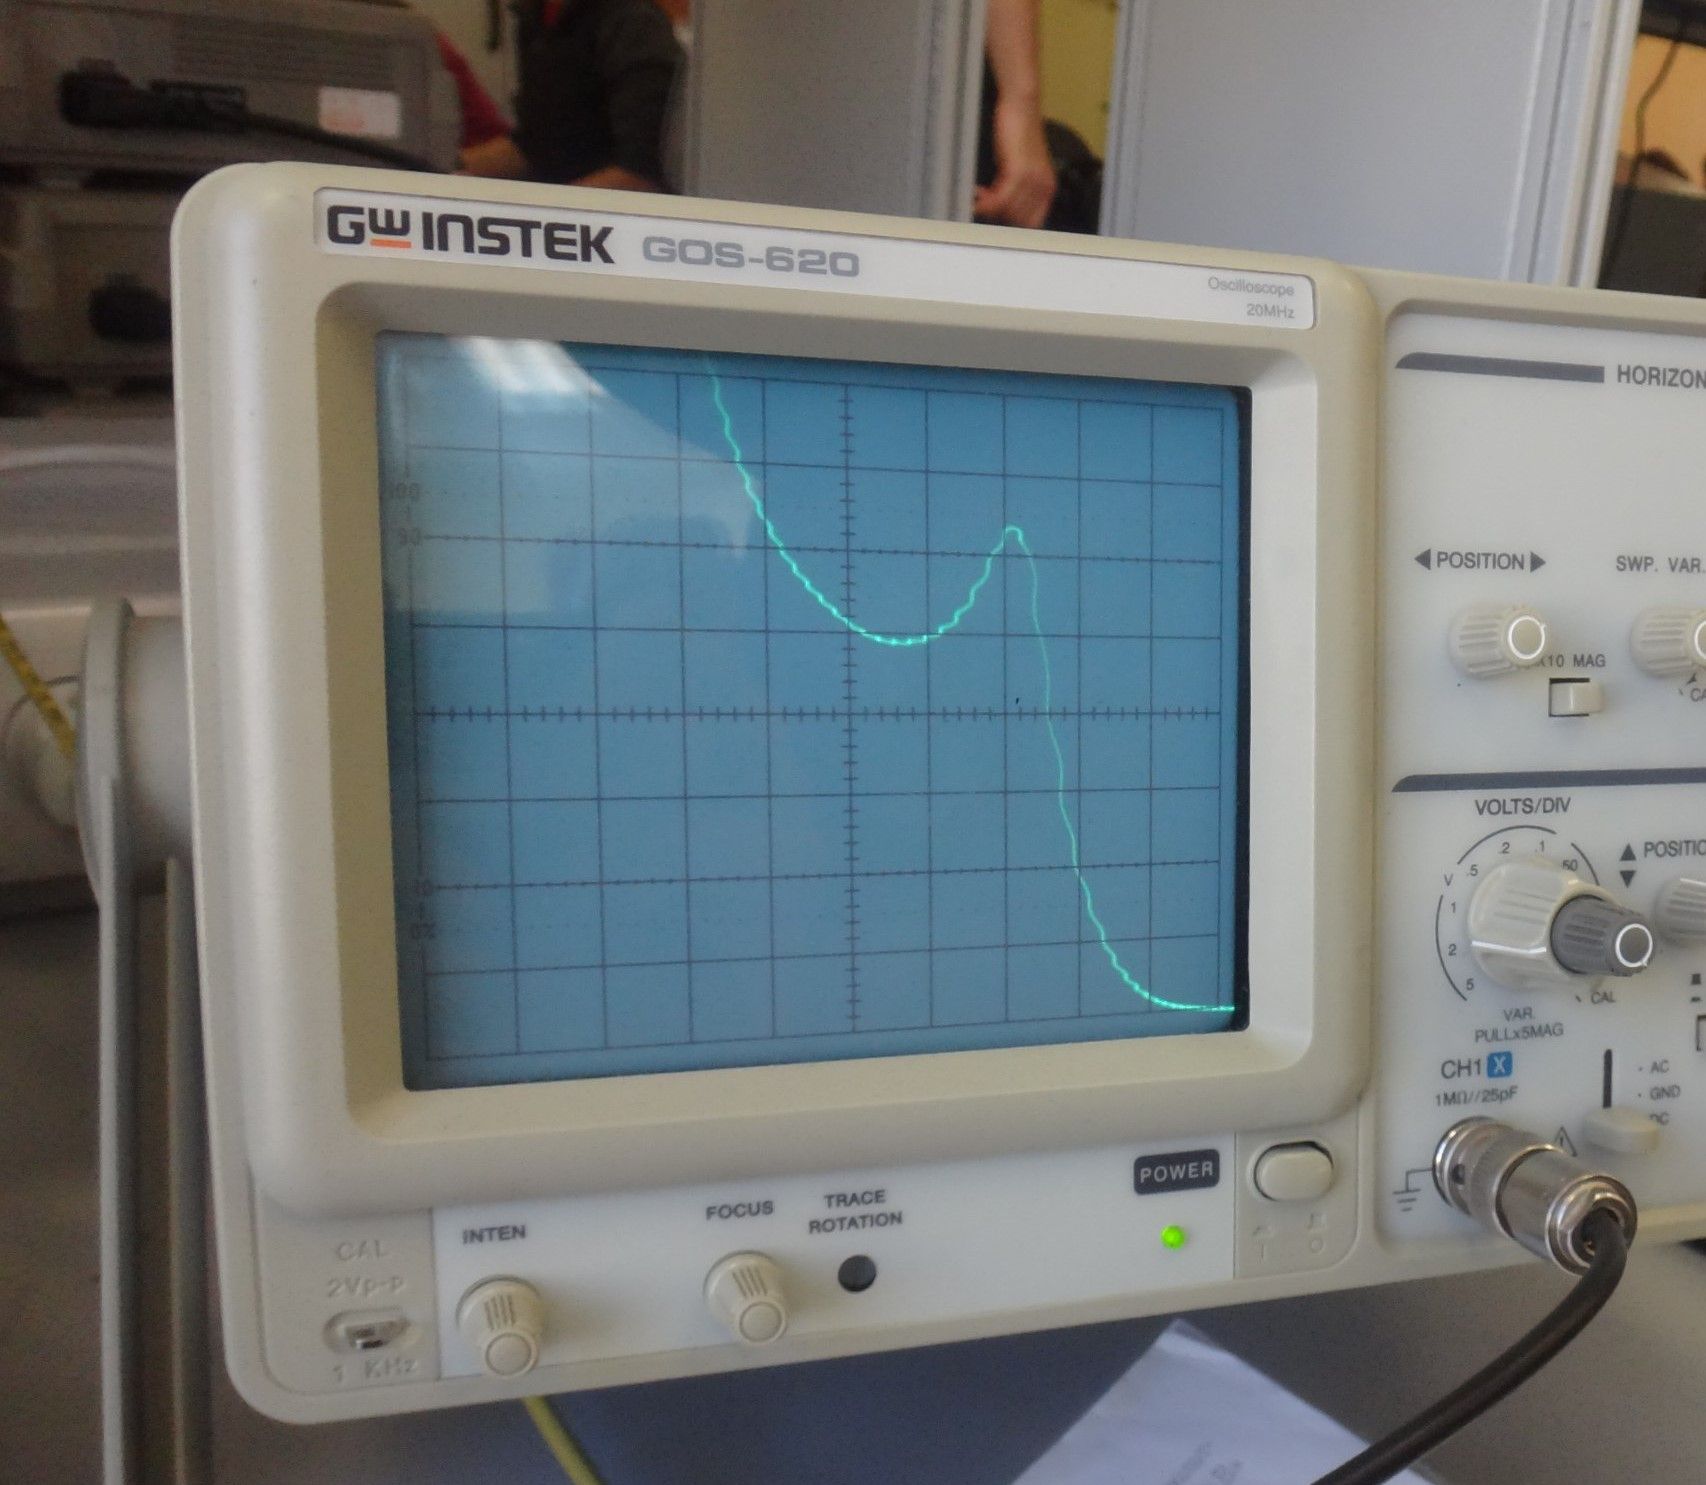
\includegraphics[width=0.9\linewidth]{osc2.jpg} \\ b)}
		\end{minipage}
		\caption{Осциллограммы: (a) $V_{накала} = 2.76~B$, (b) $V_{накала} = 2.94~B$}
		\label{fig:osc}
\end{figure}

Положение первого максимума $$ V_{max}^1 \approx 2 \;В.$$
Положение первого минимума $$ V_{min}^1 \approx 6 \; В.$$
Тогда 
\begin{equation*}\label{key}
	l = \frac{h}{\sqrt{2 m_e e^- (4.5~[B])}} \approx 2.9\; \text{\AA{}}
\end{equation*}
\begin{equation*}
	l = \frac{3}{4} \frac{h}{\sqrt{2 m_e e^- (8.5~[B])}} \approx 3.1\; \text{\AA{}}
\end{equation*}

Далее найдём радиус из формулы \eqref{eq:radius}:
\begin{equation*}\label{key}
	l = 3.4 \; \text{\AA{}}
\end{equation*}

Эффективная глубина потенциальной ямы равна
\begin{equation*}\label{key}
	U_0 = \frac{4}{5} \cdot 6 - \frac{9}{5} \cdot 2 = 1.2 \;эВ.
\end{equation*}

Так как напряжение пробоя примерно равно $ 12~B$, в колбу закачан ксенон.

\subsection{Статический режим}

Полученные данные в статическом режиме измерений представлены в таб.~\ref{tab:static}. По этим данным построим графики на рис.~\ref{fig:plot}.

\begin{table}[h!]
\begin{center}
\begin{tabular}{|cc|cc|}
\hline
\multicolumn{2}{|c|}{$V_{накала} = 2.7~B$}                        & \multicolumn{2}{c|}{$V_{накала} = 2.9~B$}                        \\ \hline
\multicolumn{1}{|c|}{$U~(I_a)$} & $V_{кc}$ & \multicolumn{1}{c|}{$U~(I_a)$} & $V_{кc}$ \\ \hline
\multicolumn{1}{|c|}{0}            & 0         & \multicolumn{1}{c|}{6,3}          & 0,324     \\ \hline
\multicolumn{1}{|c|}{4,72}         & 0,311     & \multicolumn{1}{c|}{96,9}         & 0,923     \\ \hline
\multicolumn{1}{|c|}{42,47}        & 0,701     & \multicolumn{1}{c|}{120,6}        & 1,033     \\ \hline
\multicolumn{1}{|c|}{100,4}        & 1,006     & \multicolumn{1}{c|}{167,87}       & 1,323     \\ \hline
\multicolumn{1}{|c|}{147,9}        & 1,268     & \multicolumn{1}{c|}{184,53}       & 1,502     \\ \hline
\multicolumn{1}{|c|}{178,4}        & 1,555     & \multicolumn{1}{c|}{191,52}       & 1,693     \\ \hline
\multicolumn{1}{|c|}{184,4}        & 1,692     & \multicolumn{1}{c|}{190,75}       & 1,929     \\ \hline
\multicolumn{1}{|c|}{178,2}        & 2,083     & \multicolumn{1}{c|}{181,67}       & 2,083     \\ \hline
\multicolumn{1}{|c|}{166,16}       & 2,337     & \multicolumn{1}{c|}{170,7}        & 2,306     \\ \hline
\multicolumn{1}{|c|}{151,44}       & 2,654     & \multicolumn{1}{c|}{156,75}       & 2,607     \\ \hline
\multicolumn{1}{|c|}{134,89}       & 3,159     & \multicolumn{1}{c|}{139,62}       & 3,157     \\ \hline
\multicolumn{1}{|c|}{124,85}       & 3,748     & \multicolumn{1}{c|}{131,4}        & 3,707     \\ \hline
\multicolumn{1}{|c|}{118,77}       & 4,469     & \multicolumn{1}{c|}{127,41}       & 4,267     \\ \hline
\multicolumn{1}{|c|}{117,5}        & 5,176     & \multicolumn{1}{c|}{126,77}       & 5,086     \\ \hline
\multicolumn{1}{|c|}{124,28}       & 6,077     & \multicolumn{1}{c|}{134,98}       & 5,847     \\ \hline
\multicolumn{1}{|c|}{136,22}       & 7,036     & \multicolumn{1}{c|}{148,55}       & 6,592     \\ \hline
\multicolumn{1}{|c|}{152,2}        & 7,894     & \multicolumn{1}{c|}{158,5}        & 7,019     \\ \hline
\multicolumn{1}{|c|}{175,6}        & 8,764     & \multicolumn{1}{c|}{192,96}       & 8,07      \\ \hline
\multicolumn{1}{|c|}{192,41}       & 9,224     & \multicolumn{1}{c|}{}             &           \\ \hline
\end{tabular}
\end{center}
\caption{Полученные значения в статическом режиме измерений}
\label{tab:static}
\end{table}

\newpage

\begin{figure}[h!]
\begin{center}
    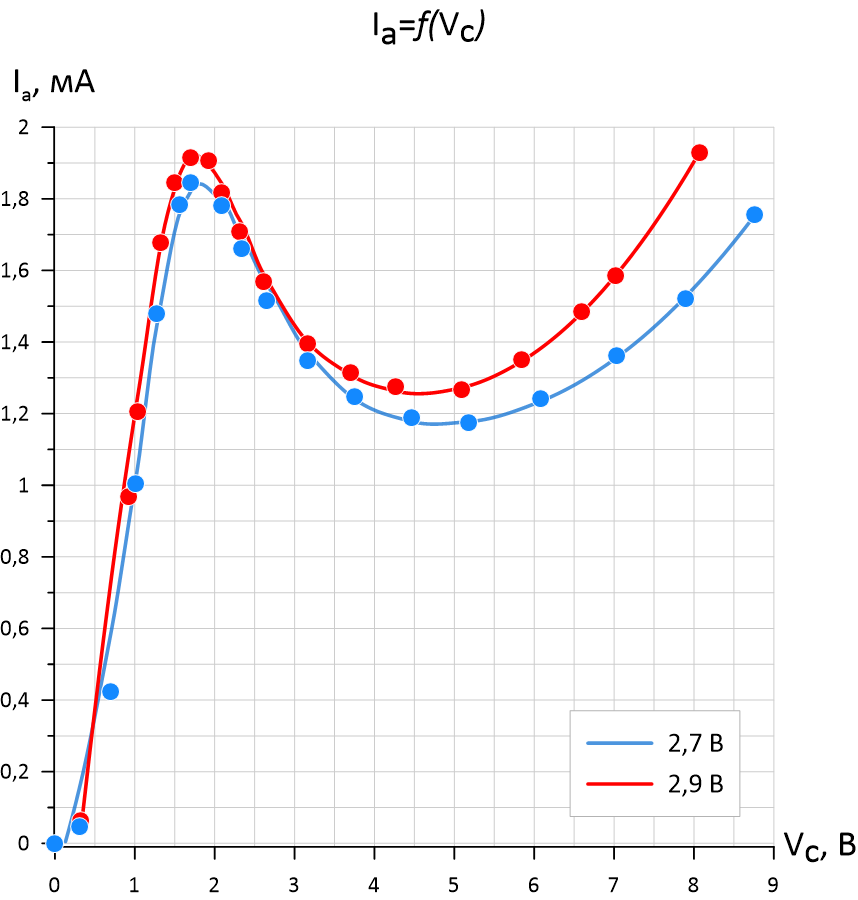
\includegraphics[width=0.6\linewidth]{plot1.png}
\end{center}
\caption{Вольт-амперная характеристика тиратрона}
\label{fig:plot}
\end{figure}

\begin{table}[h!]
	\centering
	\begin{tabular}{|l|l|l|}
	\hline
		                      & $V^1_{min}$, B        & $V^1_{max}$, B      \\ 		\hline
		$V_{накала} = 2.7\; В$ & $1.6\pm 0.1$ & $4.7\pm 0.1$ \\ 			\hline
		$V_{накала} = 2.9\; В$ & $1.7\pm 0.2$ & $4.5\pm 0.1$ \\ 			\hline
	\end{tabular}
	\caption{Результат опыта в статическом методе}
	\label{tab:stat}
\end{table}
По результатам, приведённым в табл.~\ref{tab:stat}, для $V_{накала} = 2.7\; В$:
\[
	l = 3.9 \; \text{\AA{}}; \quad U_0 = 0.88~эВ;
\]
для $V_{накала} = 2.9\; В$:
\[
	l = 4.1 \; \text{\AA{}}; \quad U_0 = 0.54~эВ.
\]

Далее по формуле \eqref{eq:at} оценим, при каких напряжениях должны появляться максимумы в коэффициенте прохождения электронов:
\[
	E = \left(\frac{\pi n \hbar}{l}\right)^2 \frac{1}{2 m} - U_0,
\]
\[  E_{n=2}= 11.7 \; эВ,\]
\[  E_{n=3} = 27.9 \; эВ. \]

Далее, по формуле \eqref{eq:probable} найдём зависимость вероятности рассеяния от энергии
\[\omega(V) \propto \ln \frac{V_{анод}}{V_{анод}^0},\] где $ V_{анод}^0 $ -- первый максимум на ВАХ тиратрона. Результат отображён на рис. \ref{fig:plot2}.

\begin{figure}[h!]
\begin{center}
    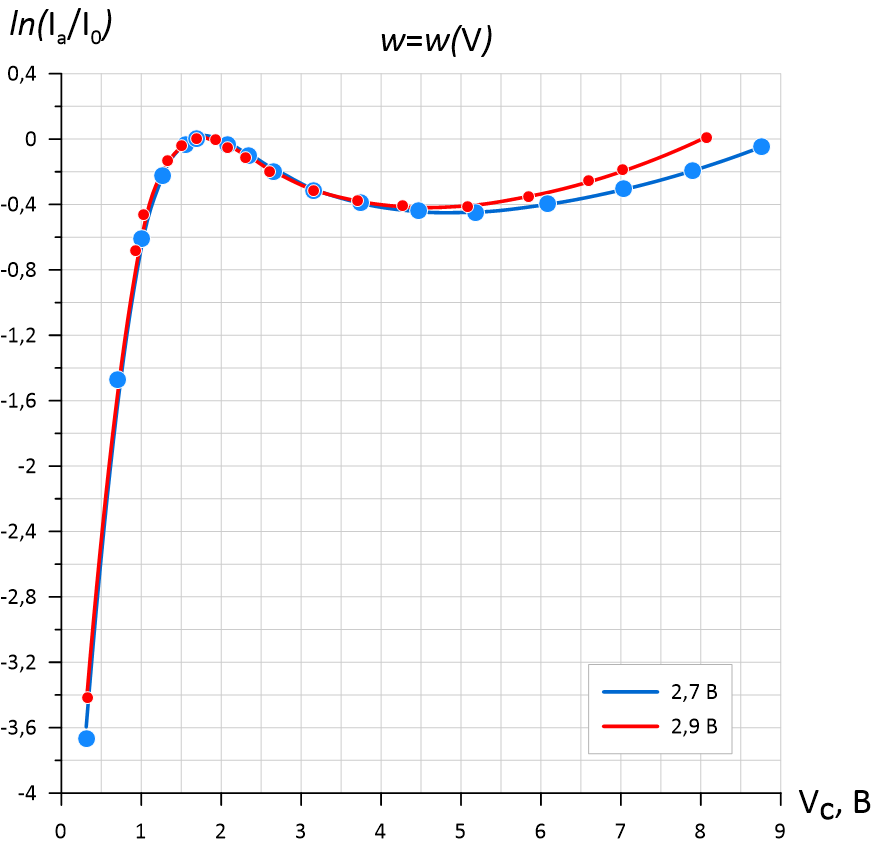
\includegraphics[width=0.6\linewidth]{plot2.png}
\end{center}
\caption{Качественный график зависимости $ \omega \propto -\ln \frac{I}{I_0} = F(V) $}
\label{fig:plot2}
\end{figure}

\newpage

\section{Обсуждение результатов и выводы}

По результатам проведения лабораторной работы установлен приблизительный радиус атома ксенона, эффективная глубина потенциальной ямы для электрона, а также получен график зависимости $ \omega = F(E) $ для вероятности рассеяния электрона.

\end{document}
